%! suppress = LineBreak
%! suppress = Unicode
%! suppress = MissingLabel
%! suppress = MissingImport
%! suppress = FileNotFound
\documentclass[../main.tex]{subfiles}

\begin{document}

    \begin{figure}[H]
        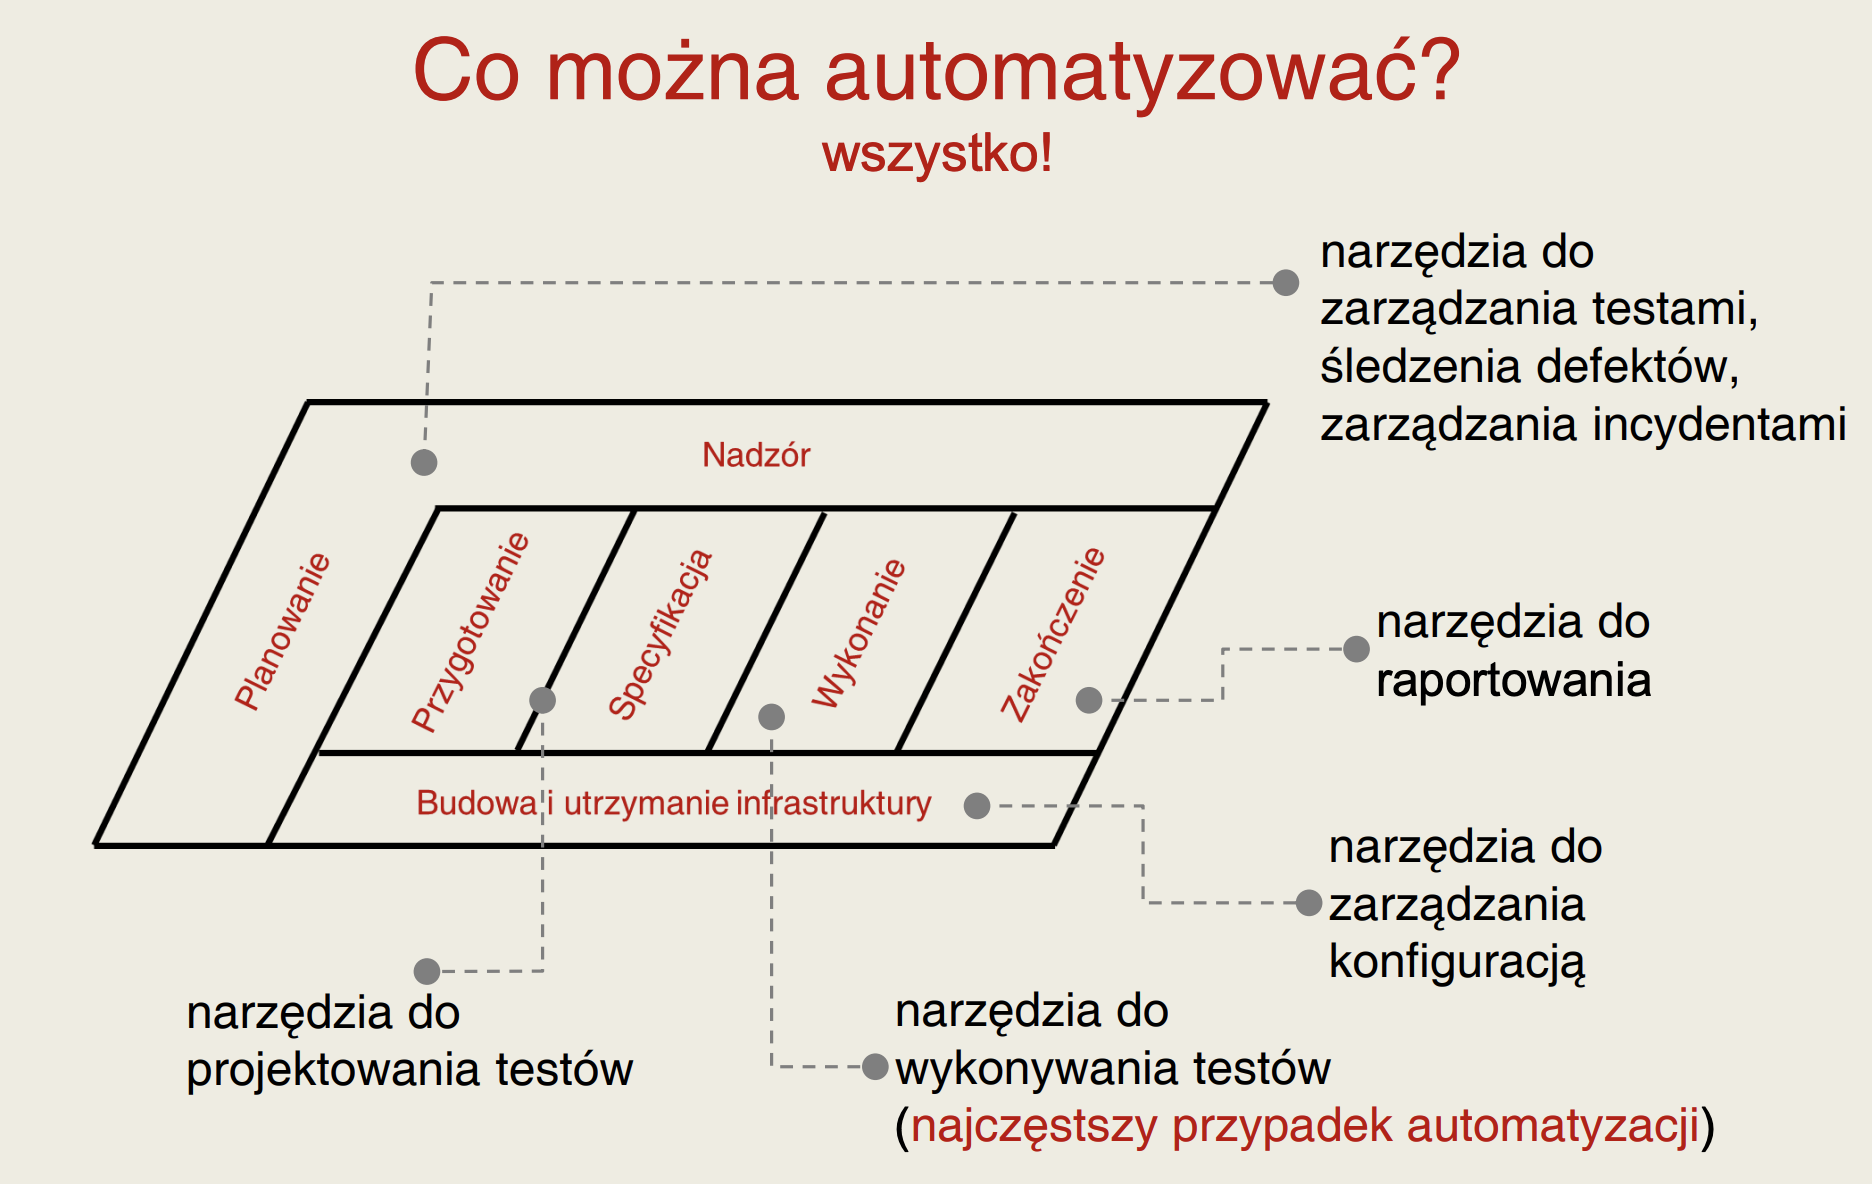
\includegraphics[width=\linewidth]{automatyzacja.png}
    \end{figure}

    \begin{figure}[H]
        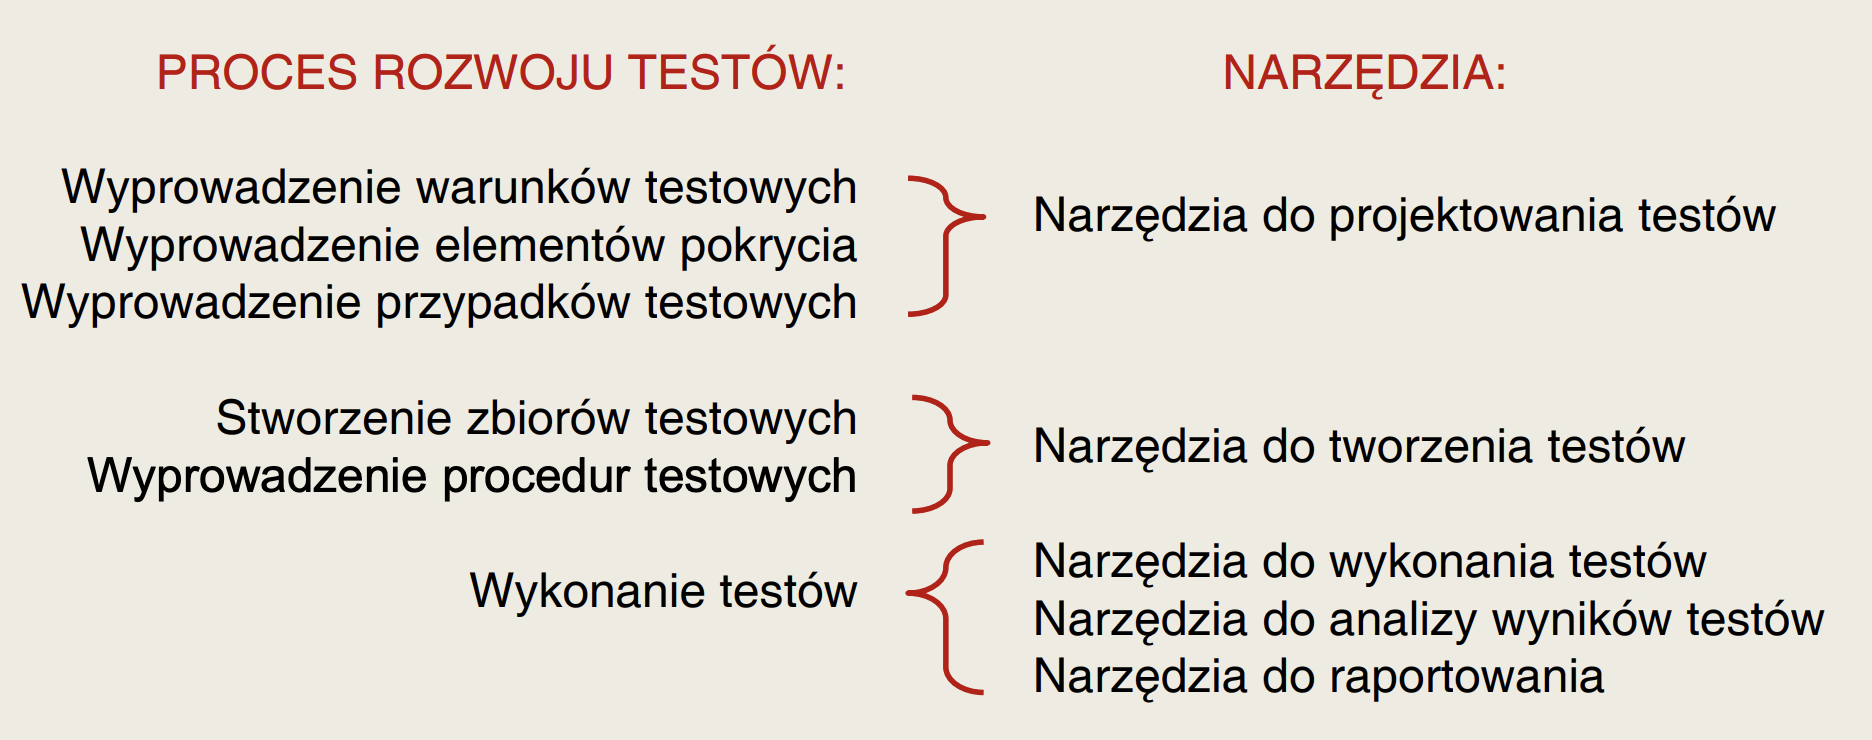
\includegraphics[width=\linewidth]{auttest.png}
    \end{figure}

    \begin{table}[H]
        \begin{center}
            \begin{tabular}{| p{8cm} | p{8cm} |}
                \hline
                \textbf{Przykładowe cele i korzyści} & \textbf{Przykładowe ryzyka} \\
                \hline
                \begin{itemize}
                    \item wykonywanie testów przez uruchamianie \textbf{skryptów}
                    \begin{itemize}
                        \item powtarzalność, spójność, efektywność
                    \end{itemize}
                    \item wykonywane testów \textbf{niemożliwych do wykonania ręcznego}
                    \begin{itemize}
                        \item np. testy wydajności, analiza statyczna
                    \end{itemize}
                    \item automatyczne \textbf{projektowanie} testów
                    \begin{itemize}
                        \item np. testy oparte na modelu
                    \end{itemize}
                    \item pomiar, analiza i raportowanie \textbf{metryk}
                    \begin{itemize}
                        \item powtarzalność, spójność, obiektywność pomiaru
                    \end{itemize}
                    \item automatyczna \textbf{generacja danych} testowych
                    \begin{itemize}
                        \item często nietrywialna
                    \end{itemize}
                    \item \textbf{porównywanie wyników} rzeczywistych z oczekiwanymi
                \end{itemize}
                &
                \begin{itemize}
                    \item \textbf{nierealistyczne oczekiwania}
                    \item \textbf{niedoszacowanie}
                    \begin{itemize}
                        \item kosztu, czasu, pracochłonności wstępnego wdrożenia
                        \item czasu i pracochłonności do osiągnięcia znaczących korzyści
                        \item pracochłonności utrzymania generowanych artefaktów
                    \end{itemize}
                    \item \textbf{zbytnie poleganie na narzędziu}
                    \item \textbf{niewykorzystanie kontroli wersji}
                    \begin{itemize}
                        \item bałagan, chaos, błędy związane z zarządzaniem konfiguracją
                    \end{itemize}
                    \item zależności i \textbf{problemy ze współpracą} krytycznych narzędzi
                    \item słaba reakcja dostawcy
                    \begin{itemize}
                        \item brak wsparcia, szkoleń itp.
                    \end{itemize}
                \end{itemize} \\
                \hline
            \end{tabular}
        \end{center}
    \end{table}


    \textbf{Efekt próbnika (probe effect)} - niezamierzony wpływ na zachowanie systemu spowodowany pomiarami tego systemu.
    Narzędzie które wpływa na wynik testu nazywamy \textbf{inwazyjnym}.

    \begin{figure}[H]
        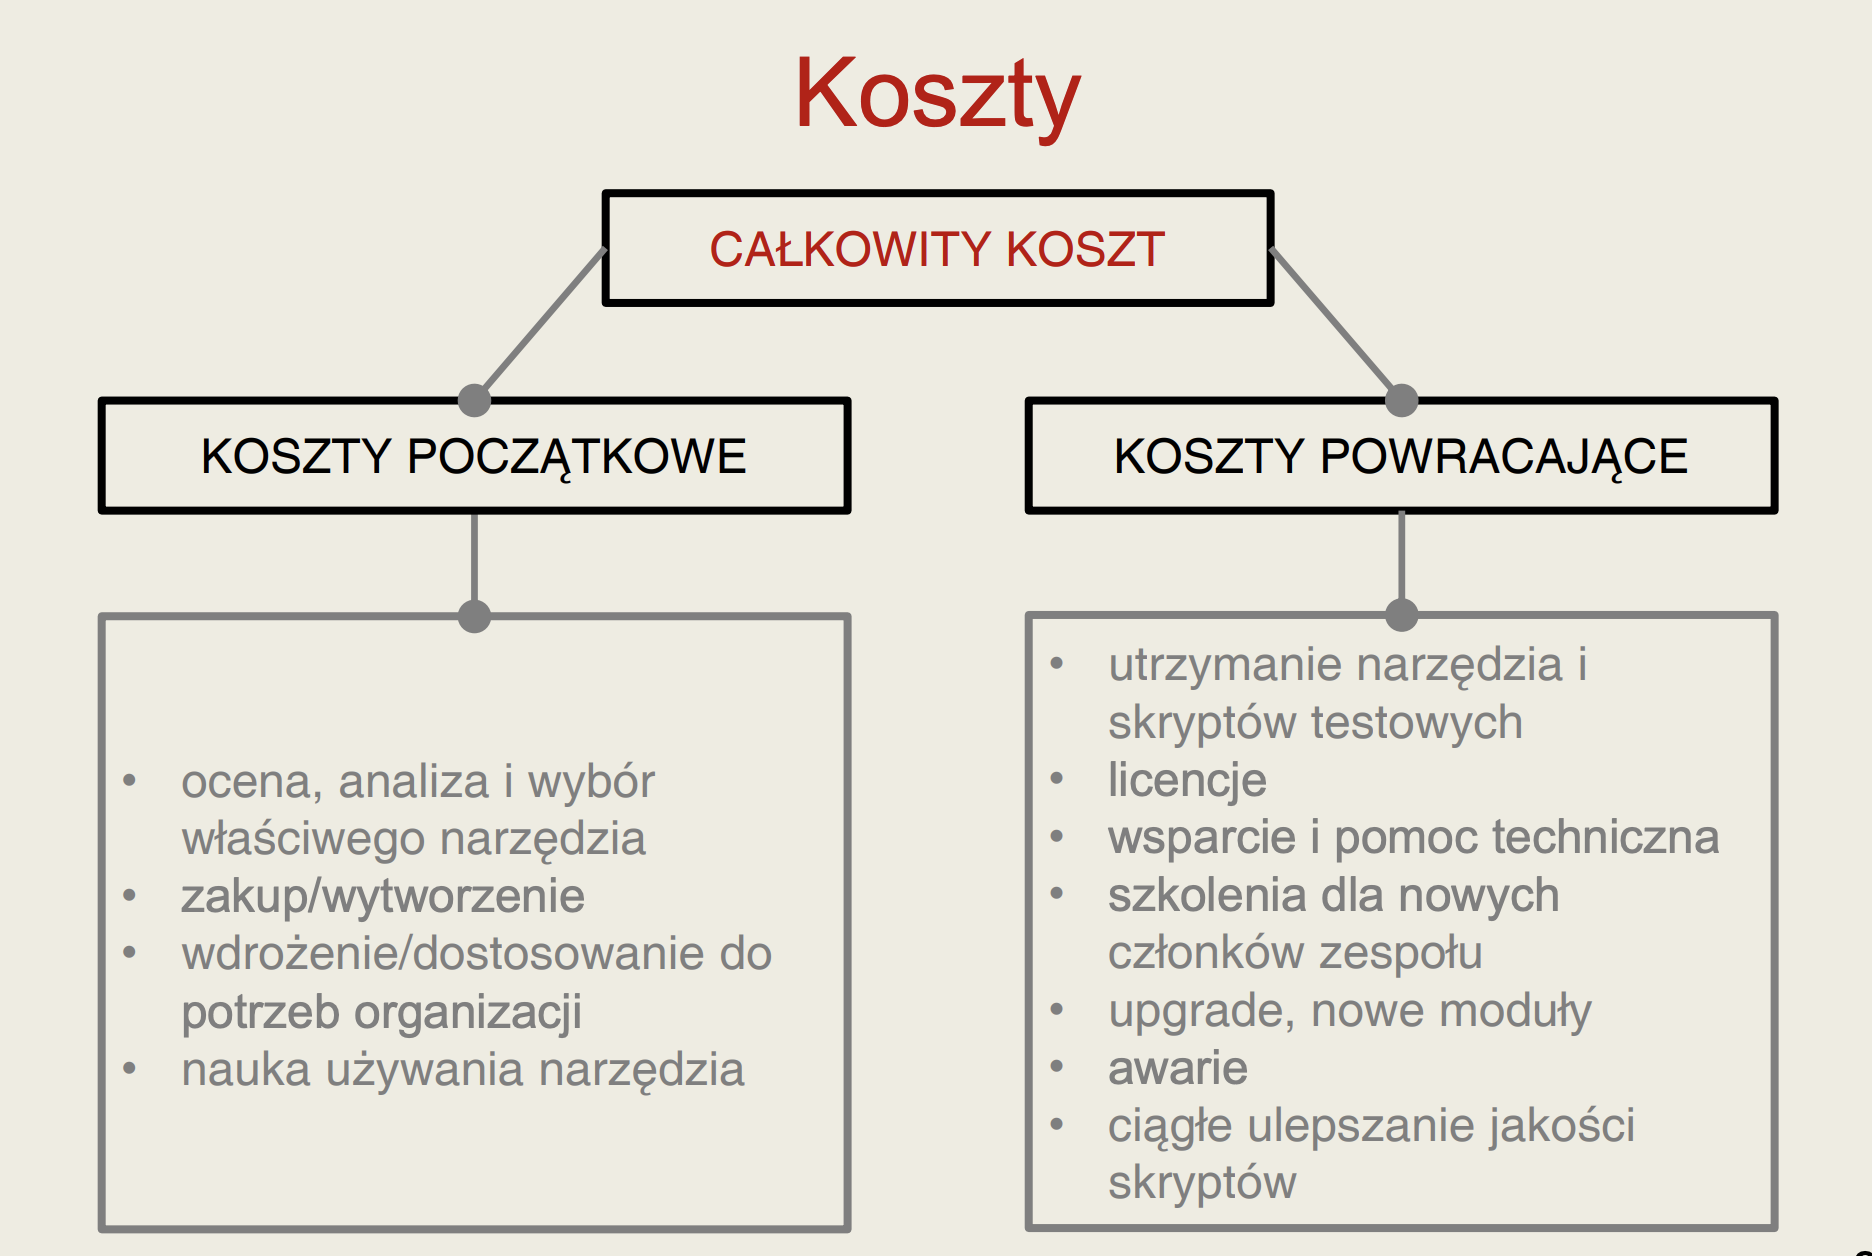
\includegraphics[width=\linewidth]{kosztaut.png}
    \end{figure}

    \subsection{Generyczna architektura automatyzacji testów}
    \begin{figure}[H]
        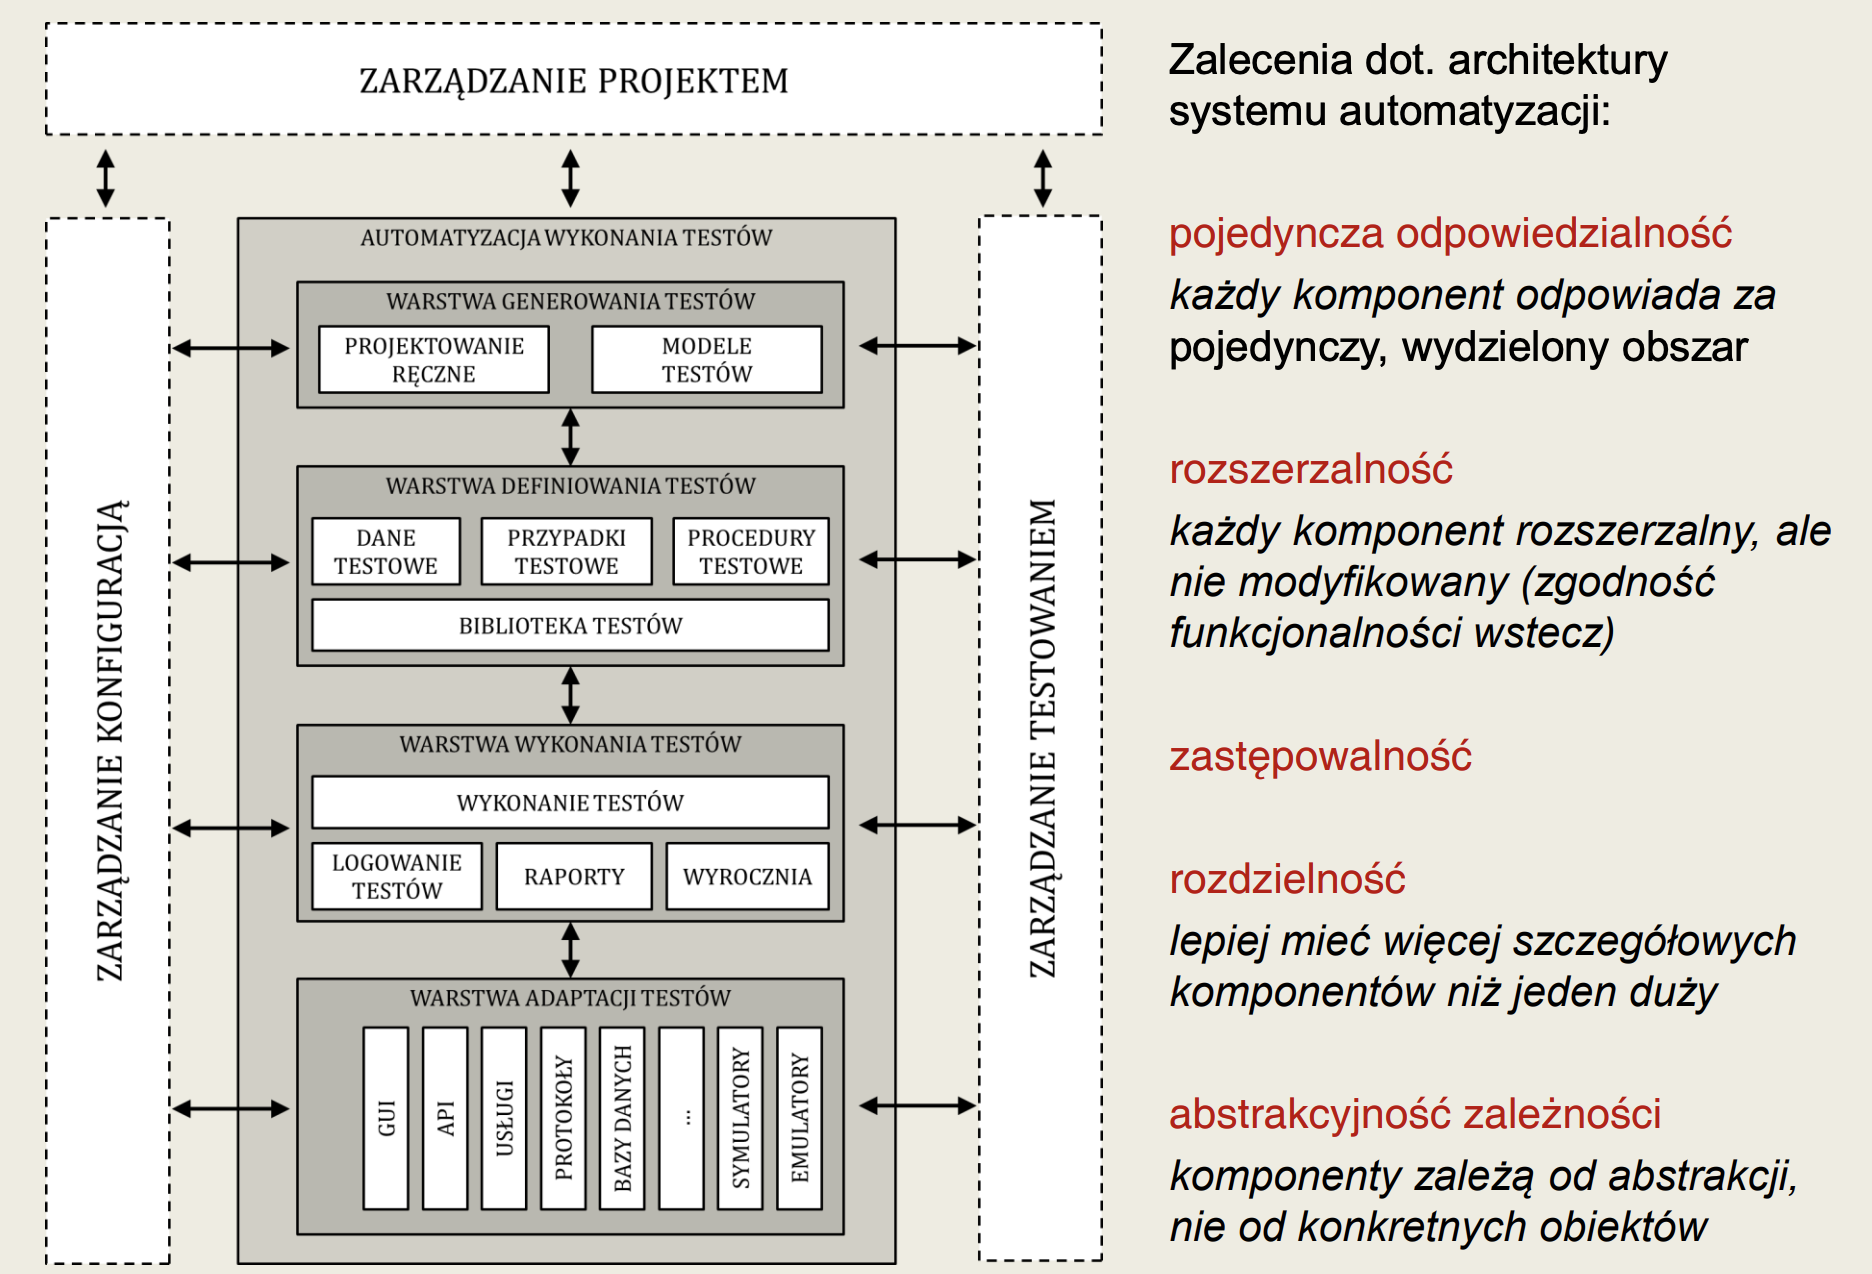
\includegraphics[width=\linewidth]{genaut.png}
    \end{figure}

    \subsection{Automatyczna generacja danych testowych}
    \begin{table}[H]
        \begin{center}
            \begin{tabular}{p{8cm} p{8cm}}
                \begin{itemize}
                    \item metoda losowa
                    \item generacja z rozkładu prawdopodobieństwa
                    \item generacja z modelu
                \end{itemize}
                &
                \begin{itemize}
                    \item generacja na podstawie symbolicznego wykonania kodu
                    \item generacja metodyczna (np. pair-wise)
                    \item generacja na podstawie danych zewnętrzych
                \end{itemize}
            \end{tabular}
        \end{center}
    \end{table}

    \subsection{Techniki automatyzacji testów}
    \begin{tabular}{| p{5cm} || p {5cm} | p{5cm} |}
        \hline
        \textbf{Technika} & \textbf{Zalety} & \textbf{Wady} \\
        \hline
        \hline
        \textbf{nagraj i odtwórz} &
        stosowalne na poziomie GUI lub API, łatwe do konfiguracji i użycia, nie
        wymaga znajomości języków
        &
        trudne w utrzymaniu, problemy gdy potrzeba czasu na odpowiedź systemu \\
        \hline
        \textbf{skrypty linearne} &
        brak żmudnych i kosztownych przygotowań, znajomość programowania niekonieczna gdy
        skrypt tworzony automatycznie
        &
        koszt automatyzacji liniowy ze względu na liczbę skryptów; trudne i kosztowne w utrzymaniu \\
        \hline
        \textbf{skrypty zorganizowane} &
        redukcja kosztów utrzymania, zmniejszenie kosztu automatyzacji nowych testów
        &
        zwiększone koszty początkowe tworzenia reużywalnych skryptów; wymaga umiejętności
        programowania \\
        \hline
        \textbf{data-driven testing} &
        niski koszt dodania testu; nie wymaga znajomości programowania; tanie w utrzymaniu
        &
        ograniczona możliwość przeprowadzania testów negatywnych \\
        \hline
        \textbf{keyword-driven testing} &
        tanie w utrzymaniu; swoboda w tworzeniu testów
        &
        kosztowna implementacja słów kluczowych; trudność w doborze właściwych słów \\
        \hline
    \end{tabular}

    \subsection{Testowanie oparte na modelu (MBT)}

    \begin{itemize}
        \item \textbf{Rozszerza i wspiera inne techniki}, takie jak np. formalne techniki projektowania testów
        \item \textbf{Podstawowa idea: ulepszyć jakość i efektywność} projektu i implementacji testów przez
        \begin{itemize}
            \item projekt wyczerpującego modelu MBT, zwykle z użyciem narzędzi, opartego na celach projektu testowego
            \item użycie modelu jako specyfikacji projektu testów, pozwalającego na automatyczną generację przypadków testowych z modelu
        \end{itemize}
        \item \textbf{Rodzaje modeli}: strukturalne, behawioralne, danych.
    \end{itemize}

    \begin{table}[H]
        \begin{center}
            \begin{tabular}{p{8cm} p{8cm}}
                \textbf{Główna motywacja: efektywność} & \textbf{Główna motywacja: wydajność} \\
                \begin{itemize}
                    \item modelowanie ułatwia \textbf{komunikację} z interesariuszami
                    \item \textbf{zrozumienie} - lepsza komunikacja pomaga stworzyć wspólną
                    płaszczyznę zrozumienia wymagań w danej dziedzinie i uniknąć potencjalnych nieporozumień
                    \item \textbf{łatwiejsze zaangażowanie} - w przypadku graficznych modeli MBT interesariusze
                    mogą być zaangażowani wcześnie
                    \item wspiera \textbf{ciągłą poprawę kompetencji} testerów
                    \item \textbf{łatwa identyfikacja „problematycznych” części systemu} - dzięki abstrakcji modeli MBT
                    \item \textbf{wczesna generacja i analiza przypadków testowych} - możliwe przed stworzeniem systemu
                \end{itemize}
                &
                \begin{itemize}
                    \item \textbf{wczesne unikanie defektów} - modele mogą być użyte do weryfikacji wymagań
                    \item \textbf{możliwe reużycie} artefaktów MBT z poprzednich projektów
                    \item \textbf{automatyzacja} - np. generacja testaliów; redukcja defektów które można
                    wprowadzić gdy testalia są tworzone i utrzymywane ręcznie
                    \item \textbf{adaptacja do zmian} - różne suity testów mogą być generowane z tego samego modelu
                    \item \textbf{uniwersalne modele} - MBT może być użyty do różnych celów testowania i do pokrycia
                    różnych poziomów i typów testów
                    \item \textbf{redukcja kosztów przy zmianie wymagań} - MBT pomaga zredukować koszty utrzymania gdy
                    zmieniają się wymagania, bo model MBT dostarcza „single point of maintenance”
                \end{itemize} \\
            \end{tabular}
        \end{center}
    \end{table}


    \begin{table}[H]
        \begin{center}
            \begin{tabular}{| p{8cm} | p{8cm} |}
                \hline
                \multicolumn{2}{|c|}{\textbf{Kryteria wyboru testów}} \\
                \hline
                \textbf{Oparte na pokryciu} & \textbf{Inne} \\
                \hline
                \begin{itemize}
                    \item \textbf{Wymagania połączone z modelem} - elementy modelu są połączone z wybranymi
                    wymaganiami. Pełne pokrycie wymagań odpowiada zestawowi testów całkowicie pokrywających wybrany zbiór wymagań.

                    \item \textbf{Elementy modelu MBT} - bazuje na \textbf{wewnętrznej strukturze modelu}. Definiuje się elementy
                    pokrycia, a testy powinny je pokrywać. Przykłady elementów pokrycia:
                    \begin{itemize}
                        \item stany, przejścia, decyzje w diagramach stanów
                        \item aktywności i bramki w modelach procesów biznesowych
                        \item warunki i akcje w tablicach decyzyjnych
                        \item instrukcje i warunki w modelach tekstualnych
                    \end{itemize}

                    \item \textbf{Oparte na danych} - związane są z takimi technikami projektowania testów jak:
                    \begin{itemize}
                        \item podział na \textbf{klasy równoważności}
                        \item analiza \textbf{wartości} brzegowych
                        \item heurystyki typu testy kombinatoryczne (np. pair-wise)
                    \end{itemize}
                \end{itemize}
                &
                \begin{itemize}
                    \item \textbf{Losowe} - polega na \textbf{losowym przechodzeniu przez model}, wszystkie przejścia są równo
                    prawdopodobne. \textbf{W podejściu stochastycznym} wybór oparty o \textbf{rozkład prawdopodobieństwa}. Model reprezentuje profil
                    użycia (tzw. \textbf{profil operacyjny}).
                    \item \textbf{Oparte na scenariuszu/wzorcu} - scenariuszem może być use case lub
                    scenariusz użycia; wzorzec = częściowo zdefiniowany scenariusz, który można
                    zastosować do modelu MBT aby wyprowadzić jeden lub wiele testów.
                    \item \textbf{Sterowane projektem} - podejście oparte na dodatkowej informacji projektowej, która została
                    dodana do modelu aby wspierać zarządzanie testami i/lub aby osiągnąć specificzne cele testowe w projekcie (np. ryzyka, priorytety).
                \end{itemize} \\
                \hline
            \end{tabular}
        \end{center}
    \end{table}

    \subsection{Wdrażanie narzędzi w organizacji}
    \begin{table}[H]
        \begin{center}
            \begin{tabular}{p{8cm} p{8cm}}
                \begin{itemize}
                    \item \textbf{ocena dojrzałości organizacji}, mocnych i słabych stron
                    \item ocena wg \textbf{jasnych wymagań} i \textbf{obiektywnych kryteriów}
                    \item wykonanie dowodu słuszności pomysłu (\textbf{proof-of-concept})
                    \item \textbf{ocena dostawcy} (w tym: szkolenia, wsparcie techniczne, aspekty komercyjne) lub firm udzielających wsparcia
                \end{itemize}
                &
                \begin{itemize}
                    \item \textbf{identyfikacja wymagań wewnętrzych} na doradztwo i szkolenia
                    \item \textbf{ocena potrzeb szkoleniowych} z uwzględnieniem obecnych umiejętności automatyzacji testów przez zespół testowy
                    \item \textbf{szacowanie} stosunku \textbf{korzyści} do \textbf{kosztów} na podstawie konkretnego przypadku biznesowego
                \end{itemize}
            \end{tabular}
        \end{center}
    \end{table}



    \begin{table}[H]
        \begin{center}
            \begin{tabular}{| p{8cm} | p{8cm} |}
                \hline
                \multicolumn{2}{|c|}{\textbf{PROJEKT PILOTAŻOWY}} \\
                \hline
                \hline
                \multicolumn{2}{|c|}{\textbf{Cele}} \\
                \hline
                \begin{itemize}
                    \item szczegółowe zaznajomienie się z narzędziem
                    \item ocena dopasowania narzędzia do obowiązujących procesów i praktyk, ustalenie co należałoby zmienić
                \end{itemize}
                &
                \begin{itemize}
                    \item ustalenie standardów użycia, zarządzania, przechowywania, pielęgnacji narzędzia i artefaktów testowych (np. konwencja nazewnictwa plików)
                    \item ocena, czy korzyści zostaną osiągnięte przy rozsądnych kosztach
                \end{itemize} \\
                \hline
                \hline
                \multicolumn{2}{|c|}{\textbf{Czynniki sukcesu}} \\
                \hline
                \begin{itemize}
                    \item stopniowe wdrażanie narzędzia w pozostałej części organizacji
                    \item adaptacja i doskonalenie procesu tak, by pasował do narzędzia
                    \item zapewnienie szkoleń i doradztwa nowym użytkownikom
                    \item zdefiniowanie wytycznych co do użycia narzędzia
                \end{itemize}
                &
                \begin{itemize}
                    \item wdrożenie sposobu na zbieranie informacji z wykorzystania narzędzia
                    \item monitorowanie wykorzystania narzędzia
                    \item monitorowanie osiąganych korzyści
                    \item zapewnienie wsparcia dla zespołu testowego w użyciu danego narzędzia
                    \item zbieranie wniosków z wykorzystania narzędzia
                \end{itemize} \\
                \hline
            \end{tabular}
        \end{center}
    \end{table}
\end{document}